\begin{exercises}
    \subsection{Bài tập}

    \begin{questions}[series=SGK]
        \item Thay dấu “?” bằng giá trị thích hợp và hoàn thành bảng sau vào vở:

        \begin{center}
            \begin{tblr}{
                width=\linewidth,
                colspec={X[1.1,c,m] X[c,m] X[c,m] X[1.35,c,m] X[1.1,c,m]},
                cells={valign=m},
                row{1}={font=\bfseries}
            }
                Hình & Bán kính đáy (cm) & Chiều cao (cm) & Diện tích xung quanh (cm$^2$) & Thể tích (cm$^3$) \\
                \SetCell[r=4]{c}
                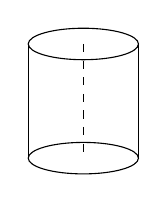
\begin{tikzpicture}
                    \coordinate (T) at (0,1.45);
                    \coordinate (B) at (0,0);
                    \draw (T) ellipse[x radius=.7,y radius=.2];
                    \draw (B) ellipse[x radius=.7,y radius=.2];
                    \draw (-.7,1.45)--(-.7,0) (.7,1.45)--(.7,0);
                    \draw[dashed] (T)--(B);
                \end{tikzpicture}
                & 4 & 6 & ? & ? \\
                & 3 & 5 & ? & ? \\
                & ? & 10 & ? & $50\pi$ \\
                & 8 & ? & $192\pi$ & ?
            \end{tblr}
        \end{center}

        \answerline
        \answerline
        \answerline

        \item Cho hình chữ nhật $ABCD$ có $AB=3$ cm, $BC=4$ cm. Quay hình chữ nhật quanh cạnh $AB$ một vòng, ta được một hình trụ. Tính diện tích xung quanh và thể tích của hình trụ tạo thành.

        \answerline
        \answerline
        \answerline

        \item Khi cho tam giác $SOA$ vuông tại $O$ quay quanh cạnh $SO$ một vòng, ta được một hình nón. Biết $OA=8$ cm, $SA=17$ cm (H.10.14).
        \begin{questions}
            \item Tính diện tích xung quanh của hình nón.
            \item Tính thể tích của hình nón.
        \end{questions}

        \begin{center}
            \begin{tikzpicture}
                \coordinate (O) at (0,0);
                \coordinate (S) at (0,3.2);
                \coordinate (A) at (1.7,0);
                \draw (S)--(O)--(A)--cycle;
                \pic[draw,angle radius=3mm] {right angle=S--O--A};
                \node[above=1pt of S] {$S$};
                \node[below left=1pt of O] {$O$};
                \node[below right=1pt of A] {$A$};
                \node[below] at ($(O)!0.5!(A)$) {$8\text{ cm}$};
                \node[right] at ($(S)!0.5!(A)$) {$17\text{ cm}$};
            \end{tikzpicture}

            \textit{Hình 10.14}
        \end{center}

        \answerline
        \answerline
        \answerline

        \item Một bóng đèn huỳnh quang có dạng hình trụ được đặt khít vào một hộp giấy cứng dạng hình hộp chữ nhật (H.10.15). Hộp giấy có chiều dài bằng $0{,}6$ m, đáy là hình vuông cạnh $4$ cm. Tính diện tích xung quanh và thể tích của bóng đèn (giả sử bề dày của hộp giấy không đáng kể).

        % TODO(HINH-NGUON): Hình 10.15 SGK trang 100 là hình phối cảnh bóng đèn trong hộp; bổ sung asset/crop đúng từ nguồn, không redraw xấp xỉ bằng TikZ.

        \answerline
        \answerline
        \answerline

        \item Một dụng cụ gồm một phần có dạng hình trụ và một phần có dạng hình nón với các kích thước như Hình 10.16.
        \begin{questions}
            \item Tính thể tích của dụng cụ này.
            \item Tính diện tích mặt ngoài của dụng cụ (không tính đáy của dụng cụ).
        \end{questions}

        \begin{center}
            \begin{tikzpicture}
                \coordinate (O0) at (0,0);
                \coordinate (O1) at (0,3.2);
                \coordinate (S) at (0,5.3);
                \coordinate (L0) at (-1.4,0);
                \coordinate (R0) at (1.4,0);
                \coordinate (L1) at (-1.4,3.2);
                \coordinate (R1) at (1.4,3.2);
                \draw (O0) ellipse[x radius=1.4,y radius=.34];
                \draw (L0)--(L1) (R0)--(R1);
                \draw (O1) ellipse[x radius=1.4,y radius=.34];
                \draw (S)--(L1) (S)--(R1);
                \draw[dashed] (S)--(O0);
                \draw (O1)--(R1);
                \node[right] at ($(O1)!0.5!(R1)$) {$40\text{ cm}$};
                \draw[<->] (1.95,0)--(1.95,3.2) node[midway,right] {$100\text{ cm}$};
                \draw[<->] (1.95,3.2)--(1.95,5.3) node[midway,right] {$50\text{ cm}$};
            \end{tikzpicture}

            \textit{Hình 10.16}
        \end{center}

        \answerline
        \answerline
        \answerline
        \answerline

        \item Tính thể tích của hình tạo thành khi cho hình $ABCD$ quay quanh $AD$ một vòng (H.10.17).

        \begin{center}
            \begin{tikzpicture}
                \coordinate (A) at (0,3);
                \coordinate (D) at (0,-6);
                \coordinate (B) at (4,3);
                \coordinate (C) at (-8,-6);
                \path[name path=AD] (A)--(D);
                \path[name path=BC] (B)--(C);
                \path[name intersections={of=AD and BC,by=X}];
                \draw (A)--(B)--(C)--(D)--cycle;
                \pic[draw,angle radius=3mm] {right angle=D--A--B};
                \pic[draw,angle radius=3mm] {right angle=C--D--A};
                \node[above left=1pt of A] {$A$};
                \node[above right=1pt of B] {$B$};
                \node[below left=1pt of C] {$C$};
                \node[below right=1pt of D] {$D$};
                \node[above] at ($(A)!0.5!(B)$) {$4\text{ cm}$};
                \node[below] at ($(C)!0.5!(D)$) {$8\text{ cm}$};
                \node[right] at ($(A)!0.5!(X)$) {$3\text{ cm}$};
                \node[right] at ($(X)!0.5!(D)$) {$6\text{ cm}$};
            \end{tikzpicture}

            \textit{Hình 10.17}
        \end{center}

        \answerline
        \answerline
        \answerline
        \answerline
    \end{questions}
\end{exercises}